\cotefile{15}
\scanpage{218}
% The typescript numbers its displayed equations at the left.
\makeatletter
\tagsleft@true
\makeatother
% archive sheet number: 217

\mspage{1 - 47 -} \hfill n\textsuperscript{o} 413

16. \uline{Mesure de Haar d'une variété de groupe}.

Conservons les notations de la fin du n\textsuperscript{o} précédent. L'espace $\Omega_e^n(G)$ est alors de dimension $1$ et il en résulte que \uline{l'espace des formes différentielles invariantes à gauche et de degré} $n=\dim G$ \uline{est de dimension} $1$. On en obtient une \uline{base} en prenant une base $\omega_1,\ldots,\omega_n$ de $\Omega_e^1(G)$ et en prenant le produit extérieur des formes $I^g_{\omega_k}$. Avec les notations de (30), on obtient en prenant $\omega_k=\mathrm{d}x_k$, l'expression d'une forme invariante à gauche $I^g_\omega$ de degré maximum au voisinage de $e$ :

\[
I^g_\omega(x)=(\text{dét}\,\partial m_k/\partial y_j(x^{-1};x))\,\mathrm{d}x_1\,\ldots\,\mathrm{d}x_n. \tag*{(31)}
\]

D'autre part, il est clair que l'espace des formes différentielles invariantes à gauche est invariant par translations à droite. Il existe donc une fonction de classe $C^{r-1}$ sur $G$, soit $\delta$, telle que :

\[
I^g_\omega(xy)=\delta(y)\,I^g_\omega\qquad (x,y\in G\,,\;\omega\in\Omega_e^n(G)). \tag*{(32)}
\]

Mais on a $\delta(y)\,I^g_\omega=I^g_\omega(xy)=I^g_\omega(y^{-1}xy)=I^g_{\omega'}$ avec $\omega'=(\operatorname{ad}y^{-1})_*(\omega)$. D'où :

\[
\delta(y)=(\text{dét}\,\operatorname{ad}y)^{-1}. \tag*{(33)}
\]

Supposons maintenant que $K$ soit \uline{localement compact} et soit $\omega\in\Omega_e^n(G)$. Il est clair que la mesure $\mu=|I^g_\omega|$ est une \uline{mesure de Haar à gauche}\unsure{.} sur le groupe localement compact $G$. Avec les notations de (30) et (31), on a donc pour $x$ voisin de $e$ :

\[
\mathrm{d}\mu(x)=\operatorname{mod}(\text{dét}\,\partial m_k/\partial y_j(x^{-1};x)))\,\mathrm{d}x_1\,\ldots\,\mathrm{d}x_n \tag*{(34)}
\]

où $\operatorname{mod}$ est le \uline{module} du corps localement compact $K$ (Int. VII, \S\ 1, n\textsuperscript{o} 10 et F. R. V.). D'autre part, (32) et (33) montrent que le \uline{module} du groupe localement compact $G$ (Int. VII, \S\ 1, n\textsuperscript{o} 3, déf. 3) n'est autre que

\[
\Delta(y)=\operatorname{mod}(\delta(y))=\operatorname{mod}(\text{dét}\,\operatorname{ad}y)^{-1}. \tag*{(35)}
\]
\scanpage{219}
% archive sheet number: 218

$X$ \deleted{\unsure{schéma}} préschéma de type fini \inserted{normal} irréductible sur corps $k$

$v,w$ deux places archimédiennes de \deleted{$k$} $X$, d'où foncteurs fibres $\unsure{\zeta|\xi}^{\unsure{\mathbb{Z}|Z}}_v,\zeta^{\mathbb{Z}}_w$. Question : \inserted{a) Quand} sont-ils isomorphes ? b) \deleted{Est-il vrai que} Quand est-il vrai que pour tte sous-catégorie \inserted{mult.} de t. f. de $M(X)$, les restrictions de ces foncteurs \unsure{à} $M_\alpha(X)$ sont isomorphes ?

Nous pouvons supposer, quitte à remplacer $k$ par \deleted{\unsure{Soient $v',w'$ les}} \unsure{sa|la} clôture alg. ds $k(X)$, que $k$ est alg. clos ds $k(X)$ [utiliser le fait $X$ \uline{normal} !] donc $X$ est \unsure{géom.\textsuperscript{t}} irréd. sur $k$. Soit \deleted{$k_0$} $k_0$ la clôture alg. de $\unsure{\mathbb{Q}|Q}$ dans $k$.

\deleted{\unsure{le corps de coïncidence des places} (\unsure{= valuations}). \unsure{induites} sur $k$,}

\deleted{\unsure{envisager}}

\inserted{\uline{Contient la clôture alg. \deleted{$E$} de $\mathbb{Q}$ dans $k$} (p. ex. $k_0$ alg. fermé dans $k$).}

\deleted{1) $k_0$ \uline{est algébriquement fermé dans $k$}. Alors}

1\textsuperscript{o}) $v,\unsure{w'|w}$ coïncident sur $k_0$.

\[
\text{a) }\zeta^{\mathbb{Z}}_v\mid M_\alpha(X)\simeq\zeta^{\mathbb{Z}}_w\mid M_\alpha(X)\qquad\text{pour }\forall\;\alpha.
\]

\diagram{\begin{tikzcd}[ampersand replacement=\&,column sep=small,row sep=small]
X_0\arrow[rr,dash]\arrow[d,dash] \& \& X\arrow[d,dash]\\
k_0\arrow[r,dash] \& \deleted{A_0}\arrow[r,dash] \& k
\end{tikzcd}}

\diagram{\begin{tikzcd}[ampersand replacement=\&,column sep=small,row sep=small,execute at end picture={
\draw[thin] ($(midbase.west)+(-.15,0)$) -- ($(highx.east)+(.1,.12)$);
\draw[thin] (midbase.west) -- ($(highx.east)+(.24,.13)$);
\draw[thin] (midbase.center) -- ($(highx.east)+(.38,.14)$);
\draw[thin] (midbase.east) -- ($(highx.east)+(.52,.15)$);
\draw[thin] ($(midbase.east)+(.15,0)$) -- ($(highx.east)+(.66,.16)$);
\draw[thin] ($(midbase.east)+(.30,0)$) -- ($(highx.east)+(.8,.14)$);
\draw[thin] (lowq.west) .. controls +(0,-.4) and +(0,-.4) .. (lowe.east) .. controls +(.8,.9) and +(.7,.55) .. (lowe.north);
}]
\& \& \deleted{\unsure{X_0}}\arrow[rr,dash] \& \& X\arrow[dd,dash]\\
\& \& |[alias=highx]|\deleted{X_0}\arrow[d,dash]\arrow[urr,dash] \& \& \\
E\arrow[r,dash]\arrow[drr,dash] \& \unsure{k_0}\arrow[r,dash]\arrow[d,dash] \& |[alias=midbase]|\deleted{\unsure{A_0}}\arrow[rr,dash]\arrow[d,dash] \& \& k\\
\& |[alias=lowq]|\deleted{\unsure{Q|\mathbb{Q}}}\arrow[rr,dash] \& A_0 \& |[alias=lowe]|\deleted{\unsure{E|\mathbb{Z}}} \&
\end{tikzcd}}

En effet, $X$ et $M_\alpha(X)$ \unsure{provient|proviennent} de $X_0$, \inserted{$M_\alpha(X_0)$} de type fini sur $A_0$, \inserted{$k_0$} \unsure{ss alg.|alg.} de type fini de $k$, /\deleted{\unsure{et}} \deleted{\unsure{$X_0\to\operatorname{Sp} A_0$ fid plat et univ.|$X_0\to\operatorname{Spec} A_0$ fid plat et univ.}, \unsure{$\operatorname{Sp} A_0\to k$}} On est ramené au cas où $k=\deleted{\unsure{E}}k_0$, où on obtient le résultat voulu grâce au groupe fondamental transcendant. \deleted{\unsure{Mais}}

b) Si \deleted{\unsure{$k\subset k_0$}} \inserted{$v$ et $w$ coïncident sur $k$,} cet argument montre que $\zeta_v^{\mathbb{Z}}\simeq\zeta_w^{\mathbb{Z}}$. \deleted{Si \unsure{$k\ne k_0$},} \inserted{Sinon,} \deleted{je pense que $\zeta_v^{\mathbb{Z}}\ne\zeta_w^{\mathbb{Z}}$, \unsure{du moins}} \inserted{mais \unsure{si on suppose que} $k$ est} \deleted{\unsure{de type}}

\margin{/\;on peut supposer $X_0\to\operatorname{Spec} A_0$ fid plat \unsure{univers\textsuperscript{t}} connexe, et $\operatorname{Spec}(A_0)\mathbin{-} k_0$ lisse connexe, donc $X_0\mathbin{-}\operatorname{Spec} k_0$ lisse connexe.}
\scanpage{220}
% archive sheet number: 219

\mspage{- 12 -} \hfill n\textsuperscript{o}370

4) Supposons $G$ unimodulaire. Soit $\mu$ une mesure de Haar sur $G$. On a

\[
\gamma(s)\mu=\delta(s)\mu=\check{\mu}=\mu. \tag*{(26)}
\]

Si $f$ est $\mu$-intégrable sur $G$, les translatées à gauche et à droite de $f$ sont $\mu$-intégrables ainsi que $\check f$, et on a

\[
\int f(sx)\,\mathrm{d}\mu(x)=\int f(xs)\,\mathrm{d}\mu(x)=\int f(x^{-1})\,\mathrm{d}\mu(x)=\int f(x)\,\mathrm{d}\mu(x). \tag*{(27)}
\]

Si $A$ est une partie $\mu$-intégrable de $G$, $sA$, $As$ et $A^{-1}$ sont $\mu$-intégrables, et

\[
\mu(sA)=\mu(As)=\mu(A^{-1})=\mu(A). \tag*{(28)}
\]

% Pale pencil traces to the left of (28).
\figure{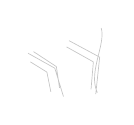
\begin{tikzpicture}[x=1cm,y=1cm,gray!45,line width=.25pt]
\draw (0,.58) -- (.34,.39) -- (.45,.03) (.07,.60) -- (.36,.41) -- (.40,.14) (.03,.47) -- (.24,.34) -- (.29,.09);
\draw (.52,.74) -- (.91,.53) -- (.86,.06) (.49,.66) -- (.83,.47) -- (.80,.12) (.88,.08) .. controls (.76,.34) and (.99,.69) .. (.93,.90);
\end{tikzpicture}}

On a des propriétés analogues pour l'intégrale essentielle.

PROPOSITION 2.- \uline{S'il existe dans} $G$ \uline{un voisinage compact} $V$ \uline{de} $e$ \uline{invariant par automorphismes intérieurs}, \uline{alors} $G$ \uline{est unimodulaire}.

En effet, soit $\mu$ une mesure de Haar à gauche sur $G$. On a, pour tout $s\in G$, $\mu(V)=\mu(s^{-1}Vs)=\Delta_G(s)\mu(V)$, d'où $\Delta_G(s)=1$ puisque $0<\mu(V)<+\infty$.

On en déduit aussitôt :

COROLLAIRE.- \uline{Si} $G$ \uline{est discret}, \uline{ou compact}, \uline{ou commutatif}, $G$ \uline{est unimodulaire}.

Ceci est d'ailleurs trivial lorsque $G$ est \uline{commutatif}. Notons aussi que, si $G$ est \uline{discret}, la mesure sur $G$ pour laquelle chaque point est de masse $1$ est évidemment une mesure de Haar à gauche et à droite sur $G$, qu'on appelle mesure de Haar \uline{normalisée} sur $G$. Si $G$ est \uline{compact}, il existe une mesure de Haar $\mu$ et une seule sur $G$ telle que $\mu(G)=1$ ; on l'appelle la mesure de Haar \uline{normalisée} de $G$. Les deux conventions précédentes ne concordent pas lorsque $G$ est à la fois discret et compact, c'est-à-dire fini ; quand on sera dans ce cas, on précisera toujours explicitement ce qu'on entend par mesure de Haar normalisée.

Un sous-groupe, un groupe quotient d'un groupe unimodulaire ne sont pas toujours unimodulaires (\S\ 2, exerc. 5). Cf., toutefois, le \S\ 2, prop. 10.

\textsuperscript{$\ast$}Nous verrons plus tard que les groupes de Lie connexes semi-simples ou nilpotents sont unimodulaires.\textsubscript{$\ast$}
\scanpage{221}
% archive sheet number: 220

\deleted{une \uline{suite} de \unsure{générateurs|génération},} \inserted{dénombrable (p. ex. de t. f. sur $\mathbb{Q}$)} on voit encore que $\unsure{\zeta|\xi}^{\unsure{\mathbb{Z}|Z}}_v\simeq\zeta_w^{\mathbb{Z}}$. En effet, $k$ est réunion filtrante d'une \uline{suite} $A_i$ de sous-$\deleted{\unsure{E}}k_0$-algèbres de type fini, on peut supposer les morphismes de transition $\operatorname{Spec} A_j\mathbin{-}\operatorname{Spec} A_i$ \unsure{lisse|lisses} à fibres géom. connexes, donc itou pour $X_j\mathbin{-}X_i$, donc aussi pour $X_{j\mathbb{C}}\mathbin{-}X_{i\mathbb{C}}$.

On a des pts $x_i,y_i$ dans $X_{i\mathbb{C}}$, s'envoyant les uns sur les autres par les morphismes de transition, et grâce à la lissité et la connexité des fibres, on voit que les morphismes de transition $\unsure{\Pi|\pi}^{1}(x_j,y_j)\mathbin{-}\Pi^{1}(x_i,y_i)$ sont surjectifs. Donc $\varprojlim_i\Pi^{1}(x_i,y_i)\ne\varnothing$, on gagne. // Si $k$ pas dénombrable,

2) \deleted{\unsure{$E\not\subset k_0$|$E\ne k_0$} \unsure{alg. fermé dans $k$|alg. fini dans $k$}.} \inserted{$v$ et $w$ ne coïncident pas sur $E$.} Alors je \deleted{\unsure{crois}} \inserted{pense} qu'il existe $\alpha$ tel que $\zeta^{\mathbb{Z}}_v\mid M_\alpha(X)\not\simeq\zeta^{\mathbb{Z}}_w\mid M_\alpha(X)$\inserted{\deleted{\unsure{de t. f.}\ \illegible{2}}}.

% slanted
\margin{\deleted{\unsure{tel que} $\unsure{\zeta_v^{\mathbb{Z}}|\xi_v^{\mathbb{Z}}}(M)\ne\unsure{\zeta_w^{\mathbb{Z}}|\xi_w^{\mathbb{Z}}}(M)$}}

On peut supposer que $X=\operatorname{Spec}\deleted{E}k$, $k$ extension finie de $\mathbb{Q}$.

\deleted{\unsure{De plus, on peut supposer}, par \unsure{descente immédiate}, que $k$ est de type fini sur $\mathbb{Q}$,}
\scanpage{222}
% archive sheet number: 221

\mspage{- 9 -} \hfill n\textsuperscript{o}370

$\mu(f')\ne0$, on a $\mu((D_f-D_{f'})g)=0$ quelle que soit $g\in\mathcal{K}$ ; remplaçant $g$ par $(D_f-D_{f'})g$, on obtient $\mu((D_f-D_{f'})^2\,g)=0$ quelle que soit $g\in\mathcal{K}^+$, donc $D_f=D_{f'}$ puisque le support de $\mu$ est $G$. Posons donc $D_f=D$. La formule (14) donne

\[
\mu(f)D(e)=\check{\nu}(f). \tag*{(17)}
\]

La formule (17) s'étend par linéarité aux $f\in\mathcal{K}$ telles que $\mu(f)=0$. On a $D(e)\ne0$ puisque $\check{\nu}\ne0$. Ceci établit bien la proportionnalité de $\mu$ et $\check{\nu}$.

COROLLAIRE.- \uline{Toute mesure complexe invariante à gauche} (resp. \uline{à droite}) \uline{sur} $G$ \uline{est proportionnelle à une mesure de Haar à gauche} (resp. \uline{à droite}).

\uline{Exemple} 1.- Sur le groupe additif $\mathbb{R}$, la mesure de Lebesgue $\mathrm{d}x$ est une mesure de Haar (Chap. III, \S\ 2; n\textsuperscript{o}2, exemple).

\uline{Exemple} 2.- Pour toute fonction $f\in\mathcal{K}(\mathbb{R}_+^*)$, on a (Fonct. var. réelles, chap. II, \S\ 1, formule (13))

\[
\int_0^{+\infty}\frac{f(x)}{x}\,\mathrm{d}x
=\int_0^{+\infty}\frac{f(tx)}{tx}\,t\mathrm{d}x
=\int_0^{+\infty}\frac{f(tx)}{x}\,\mathrm{d}x
\]

quel que soit $t>0$ ; la mesure $x^{-1}\mathrm{d}x$ est donc une mesure de Haar sur le groupe multiplicatif $\mathbb{R}_+^*$.

\uline{Exemple} 3.- Prenons pour $G$ le tore $\mathbb{T}=\mathbb{R}/\mathbb{Z}$. Soit $\varphi$ l'application canonique de $\mathbb{R}$ sur $\mathbb{T}$. Pour $f\in\mathcal{K}(\mathbb{T})$, la fonction $f\circ\varphi$ est continue et périodique de période $1$ sur $\mathbb{R}$, et l'intégrale $I(f)=\int_a^{a+1}f(\varphi(x))\mathrm{d}x$ est indépendante du choix de $a\in\mathbb{R}$ ; il est immédiat qu'elle est invariante par translation ; elle définit donc une mesure de Haar sur $\mathbb{T}$. Par transport de structure, on en déduit que $I(f)=\int_a^{a+1}f(e^{2\unsure{\text{\P}|\pi}it})\mathrm{d}t$ est une mesure de Haar sur le groupe multiplicatif $\mathbb{U}$ des nombres complexes de valeur absolue $1$ (Top. géné., chap. VIII, \S\ 2, n\textsuperscript{o}1).

PROPOSITION 1.- \uline{Soient} $G$ \uline{un groupe localement compact}, $\mu$ \uline{une mesure de Haar à gauche ou à droite sur} $G$. \uline{Pour que} $G$ \uline{soit discret}, \uline{il faut et il suffit que}
\scanpage{223}
% archive sheet number: 222

Il suffirait de construire $X$ projectif lisse sur $k$, tel que $H^{\unsure{*|\alpha}}(X_{\unsure{w|v}},\mathbb{Z})$ et $H^*(X_{\unsure{v|w|v'}},\mathbb{Z})$ non isomorphes comme \uline{anneaux}.

% slanted
\margin{Peut-on remplacer $\mathbb{Z}$ par $\mathbb{R}$ ??}

On devrait mettre Serre à contribution.

\figure{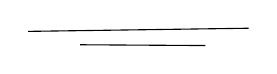
\begin{tikzpicture}[x=1cm,y=1cm]\draw (0,.17)--(2.8,.21); \draw (.66,0)--(2.25,-.01);\end{tikzpicture}}

Soit $k$ un corps de nbs, $v_0$ une place de $k$, $M$ un motif sur $k$, d'où $G_{M v_0}=G_{v_0}$ groupe algébrique \uline{défini sur} $\mathbb{Z}$. Toute autre place \deleted{\unsure{$w$}} $v$ définit un fibré principal homogène $P_v$ sous $G_{v_0}$, \unsure{et} si on admet ce qui a été \deleted{dit} \inserted{conjecturé} plus haut, \inserted{si $M$ est pris assez grand,} $v\ne v'\Longrightarrow P_v\not\simeq P_{v'}$. On peut aller plus loin et se demander si \deleted{\unsure{tout}} (pour $M$ assez grand) \uline{$\forall$} fibré principal homogène $P$ sous $G_{v_0}$ provient d'une place $v$ \deleted{\unsure{calculer|réelle}} / \deleted{\unsure{les}} On \deleted{a} peut poser

% slanted
\margin{/ Attention, la condition d'avoir un isomorphisme de foncteurs $\unsure{\zeta|\xi}(M)\otimes_{\mathbb{Z}}\mathbb{C}\simeq M_\infty\otimes_k\mathbb{C}$, satisfaisant aux conditions de compatibilité genre Riemann-Hodge, risque d'être une condition restrictive sérieuse\unsure{....|...}}

\[
G_{Mv_{\unsure{2|0|\alpha}}}(\mathbb{Z})=\unsure{\Pi|\pi}^{1}_{M}(k,v) :
\]

ces groupes à priori ne sont pas isomorphes : groupes \uline{fondamentaux \inserted{(arithmétiques)} discrets}.
\scanpage{224}
% archive sheet number: 223

\mspage{- 7 -} \hfill n\textsuperscript{o}370

si $f\leq\sum\limits_{i=1}^n c_i\gamma(s_i)g$ avec des $c_i\geq0$, on a $\sup f\leq\sum\limits_{i=1}^n c_i\,g(s_i^{-1}s)$ pour un $s\in G$, donc $\sup f\leq(\sum\limits_{i=1}^n c_i)\sup g$, d'où (iv). Prouvons (v) ; soient $f\in\mathcal{K}$, $g,h\in\mathcal{K}_+^*$ ; si $f\leq\sum\limits_{i=1}^n c_i\gamma(s_i)g$ et $g\leq\sum\limits_{j=1}^p d_j\gamma(t_j)h$ ($c_i,d_j\geq0$, $s_i,t_j\in G$), $f\leq\sum\limits_{i,j}c_i\,d_j\,\gamma(s_it_j)h$, donc $(f:h)\leq\sum\limits_{i,j}c_i\,d_j=(\sum\limits_i c_i)(\sum\limits_j d_j)$ ; donc $(f:h)\leq(f:g)(g:h)$. Si on applique (v) à $f_{\unsure{o|0}}$, $f$, $g$ d'une part et à $f$, $f_o$, $g$ d'autre part, on obtient (vi). Enfin, soient $f,f',h\in\mathcal{K}_+$ avec $h(s)\geq1$ sur le support de $f+f'$, et soit $\varepsilon>0$. Posons $F=f+f'+\frac{1}{2}\varepsilon h$ ; les fonctions $\varphi,\varphi'$, qui coïncident respectivement avec $f/F$ et $f'/F$ sur le support de $f+f'$ et qui sont nulles en dehors de celui-ci, appartiennent à $\mathcal{K}_+$ ; pour tout $\eta>0$, il existe un voisinage compact $V$ de $e$ tel que $|\varphi(s)-\varphi(t)|\leq\eta$ et $|\varphi'(s)-\varphi'(t)|\leq\eta$ pour $s^{-1}t\in V$. Soit alors $g\in\mathcal{K}_+^*(V)$ ; pour tout $s\in G$, on a $\varphi.\,\gamma(s)g\leq(\varphi(s)+\eta).\,\gamma(s)g$ (en effet, c'est évident aux points où $\gamma(s)g$ s'annule, donc hors de $sV$ ; et, dans $sV$, $\varphi\leq\varphi(s)+\eta$) ; de même, $\varphi'.\,\gamma(s)g\leq(\varphi'(s)+\eta).\,\gamma(s)g$. Ceci posé, soient $c_1,\ldots,c_n$ des nombres $\geq0$ et $s_1,\ldots,s_n$ des éléments de $G$ tels que $F\leq\sum\limits_{i=1}^n c_i\gamma(s_i)g$ ; on a

\[
f=\varphi F\leq\sum_{i=1}^n c_i\,\varphi.\,\gamma(s_i)g\leq\sum_{i=1}^n c_i(\varphi(s_i)+\eta).\,\gamma(s_i)g
\]

et de même pour $f'$ ; par suite

\[
(f:g)+(f':g)\leq\sum_{i=1}^n c_i(\varphi(s_i)+\varphi'(s_i)+2\eta)\leq(1+2\eta)\sum_{i=1}^n c_i
\]

puisque $\varphi+\varphi'\leq1$. En appliquant la définition de $F$, puis (ii), (iii), et (v), on en conclut

\[
\begin{aligned}
(f:g)+(f':g)&\leq(1+2\eta)(F:g)\leq(1+2\eta)\left[(f+f':g)+\frac{1}{2}\varepsilon(h:g)\right]\leq{}\\
&\leq(f+f':g)+\frac{1}{2}\varepsilon(h:g)+2\eta(f+f':h)(h:g)+\varepsilon\eta(h:g)
\end{aligned}
\]

et, si on a choisi $\eta$ tel que $\eta\left[2(f+f':h)+\varepsilon\right]\leq\frac{1}{2}\varepsilon$, on obtient (vii).

Quand $V$ parcourt l'ensemble des voisinages compacts de $e$, les $\mathcal{K}_+^*(V)$ forment une base de filtre $\unsure{\mathscr{B}|\mathcal{B}}$ sur $\mathcal{K}_+^*$. Soit $\unsure{\mathscr{F}|\mathcal{F}}$ un ultrafiltre sur $\mathcal{K}_+^*$ plus fin que $\mathscr{B}$.
\scanpage{225}
% archive sheet number: 224

% slanted
\margin{\deleted{$X$ \inserted{\unsure{normal irréduct.}} de type fini sur un \unsure{corps}}}

On a vu plus haut qu'une place est très loin d'être caractérisée par le foncteur fibre correspondant, \deleted{Mais} considéré comme foncteur dans les $\mathbb{Z}$-modules. Mais que se passe-t-il si on le regarde comme foncteur dans les structures de Hodge ? \deleted{Si on part} \inserted{Cela \deleted{\unsure{doit être}} est vrai pour un schéma \unsure{st local|strict local}, et pour la \unsure{même raison}}

% slanted
\margin{attention, il faut parler des \unsure{pts complexes|pl. complexes}, \unsure{ou|et non} seulement des \unsure{pl. ré. conj.}, pour pouvoir définir la structure de Hodge \unsure{---|...}}

\diagram{\begin{tikzcd}[ampersand replacement=\&,column sep=small,row sep=small,execute at end picture={
\draw[thin] (topleft.north east) -- (bottomleft.south west);
\draw[thin] ($(topleft.east)+(.07,0)$) -- ($(bottomleft.east)+(-.02,-.08)$);
\draw[thin] (bottommid.north) .. controls +(-.5,-.8) and +(-.4,.9) .. (bottomright.west);
}]
\& |[alias=topleft]|\deleted{\unsure{X_i|X_0}}\arrow[r,dash]\arrow[d,dash]\arrow[dl,dash] \& X\arrow[d,dash]\arrow[dl,dash]\\
|[alias=bottomleft]|\deleted{\unsure{\mathbb{Q}|k_0}}\arrow[r,dash] \& |[alias=bottommid]|\deleted{\unsure{A_i}}\arrow[r,dash] \& |[alias=bottomright]|k
\end{tikzcd}}

\diagram{\begin{tikzcd}[ampersand replacement=\&,row sep=small] X\arrow[d,dash]\\ {}\end{tikzcd}}

\deleted{\unsure{par-dessus le point}, on est ramené au cas où \unsure{deux places coïncident déjà sur} $k_0=$ clôture alg. de $\unsure{\mathbb{Q}|Q}$ dans $k$, et puis au cas où $X$ est de type}

\deleted{$X$ est de type fini sur \deleted{\unsure{un}} $\mathbb{Q}$, puis par \unsure{changem\textsuperscript{t}} de base au cas où $X$ est connexe de type fini sur $\mathbb{C}$, et qu'on a deux pts \inserted{ordinaires} de $X$ à val. dans $\mathbb{C}$.}

\deleted{Supposant pour simplifier que \deleted{\unsure{la courbe}} $X$ est \deleted{\unsure{réunion des}\ \illegible{1}} \deleted{affine,} quasi-projectif, \deleted{\unsure{est affine}}, on est ramené au cas où on peut supposer $X=P^{r}_{\mathbb{C}}$.}

Il semble qu'on se ramène facilement au cas de $X=\mathbb{P}^{\unsure{*|1}}_{\mathbb{C}}-(0)-(1)-(\infty)$, \inserted{et deux pts à val. ds $\mathbb{C}$ ord.,} où la théorie \unsure{classique} \deleted{\unsure{doit}} le donner --- [prendre comme motif celui défini par un schéma en courbes elliptiques sur $X$, d'invariant l'indéterminée $j$].
\scanpage{226}
% archive sheet number: 225

\mspage{- 6 -} \hfill n\textsuperscript{o}370

2. \uline{Le théorème d'existence et d'unicité}.

\figure{
\begin{tikzpicture}[x=1cm,y=1cm,gray!55,line width=.27pt]\draw (0,.12)--(.11,-.03) (.07,.14)--(.17,-.04) (.14,.15)--(.24,0) (.13,.05)--(.25,.18) (.21,.12)--(.31,.03);\end{tikzpicture}}

DÉFINITION 2.- \uline{Soit} $G$\handwritten{\unsure{$\checkmark$}} \uline{un groupe localement compact}. \uline{On appelle mesure de Haar à gauche} (resp. \uline{à droite}) \uline{sur} $G$ \uline{une mesure positive non nulle sur} $G$, \uline{invariante à gauche} (resp. \uline{à droite}).

THÉORÈME 1.- \uline{Sur tout groupe localement compact}, \uline{il existe une mesure de Haar à gauche} (resp. \uline{à droite}), \uline{et}, \uline{à un facteur constant près}, \uline{il n'en existe qu'une}.

A) \uline{Existence} - Posons $\mathcal{K}(G)=\mathcal{K}$, $\mathcal{K}_+(G)=\mathcal{K}_+$, $\mathcal{K}_+^*=\mathcal{K}_+-\{0\}$. Si $C$ est une partie compacte de $G$, on notera $\mathcal{K}_+^*(C)$ l'ensemble des $f\in\mathcal{K}_+^*$ à support dans $C$. Pour $f\in\mathcal{K}$ et $g\in\mathcal{K}_+^*$, il existe des nombres $c_1,\ldots,c_n\geq0$ et des éléments $s_1,\ldots,s_n$ de $G$ tels que $f\leq\sum\limits_{i=1}^n c_i\,\gamma(s_i)g$. (En effet, il existe une partie ouverte non vide $U$ de $G$ telle que $\inf_{s\in U}g(s)>0$, et le support de $f$ peut être recouvert par un nombre fini de translatés à gauche de $U$). Soit alors $(f:g)$ la borne inférieure des nombres $\sum\limits_{i=1}^n c_i$ pour tous les systèmes $(c_1,\ldots,c_n,s_1,\ldots,s_n)$ de nombres $\geq0$ et d'éléments de $G$ tels que $f\leq\sum\limits_{i=1}^n c_i\,\gamma(s_i)g$. On a :

\[
(\gamma(s)f:g)=(f:g)\qquad\text{pour }f\in\mathcal{K},\;g\in\mathcal{K}_+^*,\;s\in G\ ; \tag*{(i)}
\]

\[
(\lambda f:g)=\lambda(f:g)\qquad\text{pour }f\in\mathcal{K},\;g\in\mathcal{K}_+^*,\;\lambda\geq0\ ; \tag*{(ii)}
\]

\[
(f+f':g)\leq(f:g)+(f':g)\qquad\text{pour }f,f'\in\mathcal{K},\;g\in\mathcal{K}_+^*\ ; \tag*{(iii)}
\]

\[
(f:g)\geq(\sup f)/(\sup g)\qquad\text{pour }f\in\mathcal{K},\;g\in\mathcal{K}_+^*\ ; \tag*{(iv)}
\]

\[
(f:h)\leq(f:g)(g:h)\qquad\text{pour }f\in\mathcal{K},\;g,h\in\mathcal{K}_+^*\ ; \tag*{(v)}
\]

\[
0<\frac{1}{(f_{\unsure{o|0}}:f)}\leq\frac{(f:g)}{(f_o:g)}\leq(f:f_o)\qquad\text{pour }f,f_o,g\in\mathcal{K}_+^*\ ; \tag*{(vi)}
\]

\[
\begin{aligned}
&\text{soient } f,f',h\in\mathcal{K}_+\text{ avec }h(s)\geq1\text{ sur le support de }f+f',\text{ et soit}\\
&\varepsilon>0\ ;\ \text{il existe un voisinage compact }V\text{ de }e\text{ tel que, pour toute}\\
&g\in\mathcal{K}_+^*(V),\ \text{on ait }(f:g)+(f':g)\leq(f+f':g)+\varepsilon(h:g).
\end{aligned} \tag*{(vii)}
\]

Les propriétés (i), (ii), (iii) sont évidentes. Soient $f\in\mathcal{K}$, $g\in\mathcal{K}_+^*$ ;
\scanpage{227}
% archive sheet number: 226

D'autre part, \uline{quels} sont les foncteurs multiplicatifs de Motifs, à valeurs dans les structures de Hodge \inserted{(i.e. dans les motifs sur $\mathbb{C}$ !)}\margin{en vertu de la conjecture de Hodge}, qui sont associés à des places archimédiennes ? Plus généralement, dans quelle mesure un morphisme de préschémas $X\mathbin{-}Y$ est il connu par le foncteur sur les motifs \inserted{(\unsure{loc. cts|loc. ct\textsuperscript{s}|loc. cit.})}, et dans quelle mesure ce foncteur \inserted{multiplicatif} peut-il être pris arbitrairement ???

C'est lié au Pb de \uline{construire des schémas de modules} pour les motifs polarisés ; si donc $Y$ admet un motif polarisé global tel que $Y\to\text{Modules}$ est une \inserted{\unsure{imm.} (resp une\ldots} \unsure{immersion}) \deleted{et} alors cela marchera. \unsure{Kif Kif|Kif kif} si $Y$ est $\varprojlim$ de préschémas ayant cette \unsure{louable} propriété. Marchera en particulier si $Y$ est le spectre d'un corps......
\scanpage{228}
% archive sheet number: 227

\mspage{- 5 -} \hfill n\textsuperscript{o}370

On définit de manière analogue les mesures invariantes, relativement invariantes et quasi-invariantes par $G$ sur $X$. Si $\mu$ est relativement invariante, on définit son multiplicateur $\chi$ par les formules

\[
\delta(s)\mu=\chi(s)\mu \tag*{(7')}
\]

\[
\int_X f(xs)\mathrm{d}\mu(x)=\chi(s)^{-1}\int_X f(x)\mathrm{d}\mu(x) \tag*{(8')}
\]

\[
\mu(As)=\chi(s)\mu(A). \tag*{(9')}
\]

Si on considère le groupe opposé $G^o$ à $G$ comme opérant dans $X$ par $(x,s)\to xs$, $\mu$ est relativement invariante par $G^o$ de même multiplicateur $\chi$.

Soit enfin $G$ un groupe localement compact. Il opère sur lui-même par translations à gauche et à droite, suivant les formules $\gamma(s)x=sx$, $\delta(s)x=xs^{-1}$. Tout ce qui précède est applicable, et on a donc, sur $G$, les notions de mesures \uline{invariantes à gauche}, \uline{invariantes à droite}, \uline{relativement invariantes à gauche}, \uline{relativement invariantes à droite}, \uline{quasi-invariantes à gauche}, \uline{quasi-invariantes à droite} (cf., toutefois, les n\textsuperscript{os} 8 et 9).

L'application $x\to x^{-1}$ est un homéomorphisme de $G$ sur $G$. Pour toute fonction $f$ sur $G$, on définira la fonction $\check f$ sur $G$ par

\[
\check f(x)=f(x^{-1}). \tag*{(10)}
\]

Pour toute mesure $\mu$ sur $G$, on définira la mesure $\check\mu$ par

\[
\check\mu(f)=\mu(\check f)\qquad\text{pour }f\in\mathcal{K}(G). \tag*{(11)}
\]

Autrement dit

\[
\int_G f(x)\mathrm{d}\check\mu(x)=\int_G f(x^{-1})\mathrm{d}\mu(x) \tag*{(12)}
\]

Si $A$ est un ensemble $\check\mu$-intégrable, $A^{-1}$ est $\mu$-intégrable, et

\[
\check\mu(A)=\mu(A^{-1}). \tag*{(13)}
\]
